\documentclass{article}
\usepackage{neb-macros}
\usepackage{tikz}
  \usetikzlibrary{patterns}

\begin{document}

\CheapTitle{Over a UFD}

\begin{prop}
Let $R$ be a GCD domain and $p(x) \in R[x]$ primitive. Then $p(x)$ can be written as a product of irreducibles in $R[x]$ in essentially one way (up to a rearrangement and mutiplication by units).
\end{prop}

\begin{proof}
(type this)
\end{proof}

\begin{cor}
If $R$ is a UFD, then $R[x]$ is a UFD.
\end{cor}

\begin{proof}
(type this)
\end{proof}

\subsection*{Summary}

\begin{center}
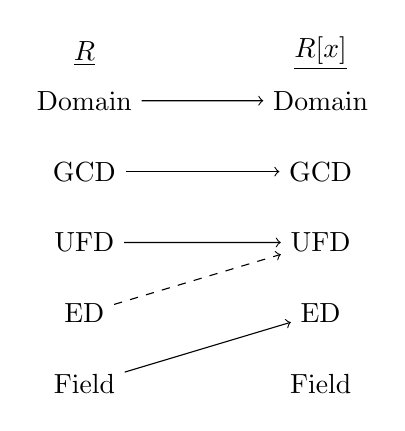
\begin{tikzpicture}[scale=0.3]
  \node (fld1) at (-5,0) {Field};
  \node (fld2) at ( 5,0) {Field};
  \node (ed1)  at (-5,3) {ED};
  \node (ed2)  at ( 5,3) {ED};
  \node (ufd1) at (-5,6) {UFD};
  \node (ufd2) at ( 5,6) {UFD};
  \node (gcd1) at (-5,9) {GCD};
  \node (gcd2) at ( 5,9) {GCD};
  \node (dom1) at (-5,12) {Domain};
  \node (dom2) at ( 5,12) {Domain};
  \node (lab1) at (-5,14) {$\underline{R}$};
  \node (lab2) at ( 5,14) {$\underline{R[x]}$};

  \draw [->] (fld1) edge (ed2);
  \draw [->, dashed] (ed1)  edge (ufd2);
  \draw [->] (ufd1) edge (ufd2);
  \draw [->] (gcd1) edge (gcd2);
  \draw [->] (dom1) edge (dom2);
\end{tikzpicture}
\end{center}

One might expect that detecting irreducibles and finding irreducible factorizations would be more difficult in $\ZZ[x]$, say, than in $\ZZ$, but in fact the opposite is true. This is ultimately due to the existence of the derivative on $R[x]$ and to some other aspects of the structure of $R[x]$ which will be explored later.

We've seen here that if $R$ is a UFD, then $R[x]$ is also a UFD, but have not seen any kind of algorithm which computes factorizations in $R[x]$. In the exercises of this and the next section we construct algorithms which work in some important special cases, including $\ZZ$ and $\ZZ/(p)$.

\subsection*{Exercises}

\begin{enumerate}
\item \textbf{Factorization if $R$ is finite.} Note that if $R$ is a finite ring of order $m$, then for any given degree $d$ there are only finitely many polynomials in $R[x]$ of degree $d$; each such polynomial has $d+1$ coefficients, which each take one of $m$ values. So the number of degree $d$ polynomials over $R$ is $m^{d+1}$.

\begin{prop}
Let $R$ be a domain. If $p(x) \in R[x]$ is reducible of degree $d$, then $p$ has a divisor of degree $1 \leq k \leq \lfloor d/2 \rfloor$.
\end{prop}

If $R$ is a finite UFD (of which examples do exist, such as $\ZZ/(p)$ with $p$ a prime) we can use this fact to construct a factorization algorithm for $R[x]$. Let $p(x) \in R[x]$ have degree $d$. Choose some $1 \leq k < d$. There are $m^{k+1}$ degree $k$ polynomials over $R$, which can easily be enumerated. (If $R$ is a field, we can consider only the monic polynomials, of which there are $m^k$.) Using polynomial long division we can determine whether any are divisors of $p(x)$; if so, recurse on the two factors, and if not, $p(x)$ has no factors of degree $k$. Repeat for each $k$ in $[1,\lfloor d/2 \rfloor]$; if no divisor of $p$ is found, then $p$ is irreducible. 
\end{enumerate}

\end{document}
